\documentclass[a4paper,11pt]{article}

\usepackage[brazil,english]{babel}
\usepackage[utf8]{inputenc}
\usepackage[T1]{fontenc}
\usepackage{anysize}
\usepackage{float}
\marginsize{2cm}{2cm}{1cm}{2cm}
\usepackage{setspace}
\setstretch{1.5}

\usepackage{graphicx}
\usepackage{amsmath,amsthm,amsfonts}
\usepackage{fancyhdr}
\usepackage{multirow}
\usepackage{footnote}
\usepackage{threeparttable}
\usepackage{rotating}
\usepackage{longtable}
\usepackage{cases}
\usepackage{mathpazo}
\usepackage{tikz}
\usepackage{indentfirst}
\usepackage{pgfplots}
\RequirePackage{lineno}
\usepackage{apacite}
\usepackage{natbib}
\bibpunct{(}{)}{;}{a}{,}{,}



\usepackage[
    a4paper,
    portuguese,
    bookmarks=true,
    bookmarksnumbered=true,
    linktocpage,
    colorlinks,
    citecolor=blue,
    plainpages=false,
    pdfpagelabels]{hyperref}

    \usepackage{listings}
\usepackage{xcolor}

\lstdefinestyle{pythonstyle}{
    language=Python,
    basicstyle=\ttfamily\footnotesize,
    keywordstyle=\color{blue},
    commentstyle=\color{gray},
    stringstyle=\color{red!60!black},
    numbers=left,
    numberstyle=\tiny,
    stepnumber=1,
    numbersep=8pt,
    showstringspaces=false,
    breaklines=true,
    frame=single,
    tabsize=4,
    captionpos=b
}

% Definições
\newtheorem{definition}{Definição}
\newtheorem{problem}{Problema}
\newtheorem{proposition}{Proposição}

% Variáveis matemáticas
\newcommand{\CC}{\mathcal{C}}
\newcommand{\CD}{\mathcal{C_D}}
\newcommand{\Cl}{\mathcal{C}^{'}}
\newcommand{\ClD}{\mathcal{C}^{'}_D}
\newcommand{\D}{\mathcal{D}}
\newcommand{\Dl}{\mathcal{D}^{'}}
\newcommand{\DlF}{\mathcal{D}^{'}_F}
\newcommand{\Dlc}{\mathcal{D}^{'}_c}
\newcommand{\F}{\mathcal{F}}
\newcommand{\Fl}{\mathcal{F}^{'}}
\newcommand{\Flc}{\mathcal{F}^{'}_c}
\newcommand{\Fli}{\mathcal{F}^{'}_i}
\newcommand{\Flt}{\mathcal{F}^{'}_t}
\newcommand{\GG}{\mathcal{G}}
\newcommand{\I}{\mathcal{I}}
\newcommand{\Il}{\mathcal{I}^{'}}
\newcommand{\IlF}{\mathcal{I}^{'}_F}
\newcommand{\M}{\mathcal{M}}
\newcommand{\Or}{\mathcal{O}}
\newcommand{\R}{\mathcal{R}}
\newcommand{\Real}{\mathbb R}
\newcommand{\Inteiro}{\mathbb Z}

\pagestyle{empty}

\title{Trabalho Final}

\author{\textbf{Autor 1 - Italo Leal Lana Santos}\\\textbf{Autor 2 - Italo Rodrigues de Matos Avelar}\\\textbf{Autor 3 - Nathan Filipe Izidorio Alves}\\\textbf{Autor 4 - Vitor Gabriel da Silva Pereira}\\\textbf{Autor 5 - Vitor Hugo Dias Santos}}
\date{\empty}

\begin{document}
\maketitle
\thispagestyle{empty}
\selectlanguage{brazil}
% =========================================
\section{Cenário 1 - Cenário Base}
% =========================================

\subsection{Base Custos Totais e Componentes}

O modelo encontrou uma solução ótima para o cenário base com um custo total de R\$ 20.501,43[cite: 3]. A distribuição dos custos indica que a maior parcela dos gastos está concentrada no processamento do café, seguido pelos custos fixos de instalação[cite: 4].

\begin{table}[H]
\centering
\begin{tabular}{lc}
\hline
\textbf{Componente de Custo} & \textbf{Valor (R\$)} \\ \hline
Processamento (Torrefadoras) & 13.110,56 \\
Instalação de CDs & 6.000,00 \\
Transporte CD $\rightarrow$ Cliente & 736,30 \\
Transporte Fornecedor $\rightarrow$ CD & 654,57 \\
Penalidade de Estoque & 0,00 \\ \hline
\textbf{Custo Total} & \textbf{20.501,43} \\ \hline
\end{tabular}
\caption{Componentes de custo no Cenário Base [cite: 5]}
\label{tab:cenario1_custos}
\end{table}

\subsection{Cidades Selecionadas e Torrefadoras}

A otimização determinou a abertura de dois Centros de Distribuição[cite: 7]:
\begin{itemize}
    \item \textbf{CD Araxá}: Instalado e operando com a torrefadora T2[cite: 8].
    \item \textbf{CD Belo Horizonte}: Instalado e operando com a torrefadora T1[cite: 9].
\end{itemize}

\subsection{Distribuição de Fluxo (Captação de Fornecedores)}

A Tabela \ref{tab:cenario1_forn_cd} apresenta a alocação dos fluxos de entrada (inbound) originados nos fornecedores com destino aos CDs abertos.

\begin{table}[H]
\centering
\begin{tabular}{lcc}
\hline
\textbf{Origem (Fornecedor)} & \textbf{Destino (CD)} & \textbf{Volume (kg)} \\ \hline
Ituiutaba & Araxá & 159,00 \\
Uberaba & Araxá & 170,00 \\
Patos de Minas & Araxá & 127,00 \\
Araxá & Araxá & 148,00 \\
São João del-Rei & Belo Horizonte & 251,00 \\
Governador Valadares & Belo Horizonte & 313,00 \\
Patos de Minas & Belo Horizonte & 5,00 \\
Barbacena & Belo Horizonte & 173,00 \\
Lavras & Belo Horizonte & 157,00 \\
Manhuaçu & Belo Horizonte & 271,00 \\
Divinópolis & Belo Horizonte & 288,00 \\ \hline
\end{tabular}
\caption{Distribuição de fluxo dos Fornecedores para os CDs [cite: 11, 13]}
\label{tab:cenario1_forn_cd}
\end{table}

\subsection{Distribuição de Fluxo (Entrega aos Clientes)}

As tabelas \ref{tab:cenario1_cd_cli_araxa} e \ref{tab:cenario1_cd_cli_bh} detalham a etapa de escoamento (outbound) dos produtos processados nos centros de distribuição até os clientes finais.

\begin{table}[H]
\centering
\begin{tabular}{lcc}
\hline
\textbf{Origem (CD)} & \textbf{Destino (Cliente)} & \textbf{Volume (kg)} \\ \hline
Araxá & Ituiutaba & 64,00 \\
Araxá & Uberaba & 121,00 \\
Araxá & Patos de Minas & 110,00 \\
Araxá & Araxá & 124,00 \\
Araxá & Alfenas & 61,00 \\
Araxá & Uberlândia & 73,00 \\
Araxá & Poços de Caldas & 51,00 \\ \hline
\end{tabular}
\caption{Distribuição de fluxo do CD Araxá para os Clientes [cite: 15]}
\label{tab:cenario1_cd_cli_araxa}
\end{table}

\begin{table}[H]
\centering
\begin{tabular}{lcc}
\hline
\textbf{Origem (CD)} & \textbf{Destino (Cliente)} & \textbf{Volume (kg)} \\ \hline
Belo Horizonte & São João del-Rei & 101,00 \\
Belo Horizonte & Governador Valadares & 142,00 \\
Belo Horizonte & Barbacena & 70,00 \\
Belo Horizonte & Lavras & 132,00 \\
Belo Horizonte & Manhuaçu & 136,00 \\
Belo Horizonte & Divinópolis & 124,00 \\
Belo Horizonte & Alfenas & 76,00 \\
Belo Horizonte & Varginha & 149,00 \\
Belo Horizonte & Ipatinga & 52,00 \\
Belo Horizonte & Juiz de Fora & 71,00 \\
Belo Horizonte & Sete Lagoas & 102,00 \\
Belo Horizonte & Teófilo Otoni & 137,00 \\
Belo Horizonte & Belo Horizonte & 79,00 \\
Belo Horizonte & Montes Claros & 87,00 \\ \hline
\end{tabular}
\caption{Distribuição de fluxo do CD Belo Horizonte para os Clientes [cite: 15, 16, 17]}
\label{tab:cenario1_cd_cli_bh}
\end{table}

\subsection{Mapa de Rotas Geradas}

A representação visual na Figura \ref{fig:mapa_cenario_base} ilustra as rotas de transporte entre fornecedores, os dois CDs instalados e os clientes finais, evidenciando a regionalização da operação logística descrita a seguir[cite: 42].

\begin{figure}[H]
\centering
\includegraphics[width=0.95\textwidth]{imgs/mapa_cenario_base.png}
\caption{Rotas logísticas geradas no cenário base [cite: 18]}
\label{fig:mapa_cenario_base}
\end{figure}

\subsection{Análise Crítica do Cenário Base}

A configuração gerada atende integralmente à demanda sem gerar estoques não distribuídos (custo de penalidade igual a zero)[cite: 44]. Dos 3 CDs permitidos pela restrição do modelo, o sistema optou por instalar apenas 2 (Araxá e Belo Horizonte)[cite: 45]. Isso demonstra que a capacidade conjunta das torrefadoras T1 e T2 nestes locais é suficiente para processar toda a oferta disponível e atender a demanda exigida, evitando o custo fixo de instalação de um terceiro centro de distribuição[cite: 46].

Os custos de processamento representam a maior proporção do custo total da rede (R\$ 13.110,56), configurando o fator mais crítico da função objetivo[cite: 47]. Os custos logísticos de transporte, tanto na captação quanto na distribuição, mantiveram-se otimizados e com impacto financeiro reduzido (R\$ 1.390,87 somados)[cite: 48, 49].

Observa-se, conforme ilustrado no mapa de rotas, uma nítida regionalização na topologia da rede[cite: 50]. O CD Araxá concentra as operações de captação e distribuição do Triângulo Mineiro e Alto Paranaíba (Ituiutaba, Uberaba, Patos de Minas, Uberlândia)[cite: 51, 52]. Por outro lado, o CD Belo Horizonte opera como o polo logístico central do estado, recebendo a carga das demais regiões produtoras e garantindo o abastecimento do Sul de Minas, Zona da Mata, Vale do Rio Doces, região Central e Norte de Minas[cite: 52].

Do ponto de vista operacional, ocorre o fracionamento pontual de cargas para otimização exata[cite: 53]. A cidade de Alfenas tem sua demanda atendida por ambos os CDs (61 kg oriundos de Araxá e 76 kg de Belo Horizonte)[cite: 54]. A captação em Patos de Minas também é dividida: a maior parte (127 kg) segue para Araxá, enquanto um pequeno resíduo (5 kg) é transportado para Belo Horizonte[cite: 55]. Esse comportamento reflete a precisão matemática do modelo em equalizar as capacidades das torrefadoras e minimizar as distâncias rodoviárias de forma global[cite: 56].

\newpage
% =========================================
\section{Cenário 2 - Aumento da Oferta}
% =========================================

O Cenário 2 avalia a resposta da malha logística a um aumento de 50\% na capacidade de oferta de todos os fornecedores, mantendo a demanda dos clientes constante e idêntica ao cenário base (2062,00 kg no total). Como consequência do aumento, a oferta total disponível na rede salta de 2062,00 kg para 3093,00 kg.

A imposição de processamento total da oferta (Equação 3) em conjunto com a igualdade estrita no atendimento da demanda (Equação 5) cria um desbalanceamento operacional: todo o café ofertado deve ser obrigatoriamente coletado e processado, restando um volume excedente de 1031,00 kg que não pode ser entregue aos clientes e deve ser retido nos Centros de Distribuição.

A Tabela \ref{tab:cenario2_custos} apresenta os custos da operação sob este cenário. Nota-se um crescimento dramático no custo total da cadeia, impulsionado pela penalidade por estocagem que representa mais de 78\% do gasto total.

\begin{table}[H]
\centering
\begin{tabular}{lccc}
\hline
\textbf{Componente de Custo} & \textbf{Valor (R\$)} & \textbf{Representatividade (\%)} \\ \hline
Custo Total             & 131135,96  & 100\%     \\
Penalidade de Estoque   & 103100,00  & $\sim$78,6\%  \\
Processamento (Torr)    &  20846,82  & $\sim$15,9\%  \\
Instalação de CDs       &   6000,00  & $\sim$4,6\%  \\
Transporte Forn->CD     &    700,71  & $\sim$0,5\%  \\
Transporte CD->Cli      &    488,43  & $\sim$0,4\%    \\
\hline
\end{tabular}
\caption{Resultados Financeiros do Cenário 2}
\label{tab:cenario2_custos}
\end{table}

\subsection{Configuração da Rede e Bottlenecks de Capacidade}

Diferente do cenário base, a rede agora opera com a abertura de um único Centro de Distribuição em Divinópolis ($w_{Divinopolis} = 2,0$), o qual foi expandido para dois módulos a fim de comportar a alocação de duas torrefadoras: T2 e T3 ($z_{Divinopolis, T2} = 1$ e $z_{Divinopolis, T3} = 1$). A Tabela \ref{tab:cenario2_cds} demonstra o balanço de fluxos no polo de Divinópolis.

\begin{table}[H]
\centering
\begin{tabular}{llrrr}
\hline
\textbf{CD aberto} & \textbf{Torrefadora} & \textbf{Entrada (kg)} & \textbf{Saída (kg)} & \textbf{Estoque (kg)} \\ \hline
Divinópolis & T2 e T3 & 3093,00 & 2062,00 & 1031,00 \\ \hline
\end{tabular}
\caption{CDs abertos, torrefadoras e balanço de fluxo no Cenário 2}
\label{tab:cenario2_cds}
\end{table}

A escolha das torrefadoras T2 e T3 é um comportamento puramente ditado pelas restrições de capacidade do modelo. Com o aumento da oferta total para 3093,00 kg, e devido à restrição de limite máximo de 2 CDs ativos ($m \le 2$), a empresa pode alocar no máximo duas torrefadoras (uma para cada módulo de CD ou divididas). A soma das capacidades de quaisquer duas torrefadoras deve suportar os 3093,00 kg de entrada:
\begin{itemize}
    \item $q_{T1} + q_{T2} = 1458 + 1580 = 3038 \text{ kg} < 3093 \text{ kg}$ (Inviável)
    \item $q_{T1} + q_{T3} = 1458 + 1587 = 3045 \text{ kg} < 3093 \text{ kg}$ (Inviável)
    \item $q_{T2} + q_{T3} = 1580 + 1587 = 3167 \text{ kg} \ge 3093 \text{ kg}$ (Viável)
\end{itemize}

Assim, o solver é matematicamente forçado a escolher T2 e T3, as duas maiores torrefadoras, descartando a torrefadora T1 que, apesar de ser a mais barata (6,20 R\$/kg) e mais rápida, gera um gargalo físico insuperável neste cenário de oferta elevada. O processamento por T2 e T3 encarece o custo de processamento total (R\$ 20.846,82).

A Tabela \ref{tab:cenario2_forn_cd} e a Tabela \ref{tab:cenario2_cd_cli} detalham os fluxos de abastecimento e distribuição da malha, respectivamente. Para a estimativa de viagens, considerou-se caminhões de capacidade padrão (500 kg), com arredondamento para cima.

\begin{table}[H]
\centering
\begin{tabular}{llcc}
\hline
\textbf{Origem (Fornecedor)} & \textbf{Destino (CD)} & \textbf{Quantidade (kg)} & \textbf{Viagens} \\ \hline
São João del-Rei & Divinópolis & 376,50 & 1 \\
Governador Valadares & Divinópolis & 469,50 & 1 \\
Ituiutaba & Divinópolis & 238,50 & 1 \\
Uberaba & Divinópolis & 255,00 & 1 \\
Patos de Minas & Divinópolis & 198,00 & 1 \\
Barbacena & Divinópolis & 259,50 & 1 \\
Lavras & Divinópolis & 235,50 & 1 \\
Manhuaçu & Divinópolis & 406,50 & 1 \\
Divinópolis & Divinópolis & 432,00 & 1 \\
Araxá & Divinópolis & 222,00 & 1 \\ \hline
\textbf{Total} & & \textbf{3093,00} & \textbf{10} \\
\hline
\end{tabular}
\caption{Distribuição dos fornecedores para os CDs no Cenário 2}
\label{tab:cenario2_forn_cd}
\end{table}

\begin{table}[H]
\centering
\begin{tabular}{llcc}
\hline
\textbf{Origem (CD)} & \textbf{Destino (Cliente)} & \textbf{Quantidade (kg)} & \textbf{Viagens} \\ \hline
CD Divinópolis & São João del-Rei & 101,00 & 1 \\
CD Divinópolis & Governador Valadares & 142,00 & 1 \\
CD Divinópolis & Ituiutaba & 64,00 & 1 \\
CD Divinópolis & Uberaba & 121,00 & 1 \\
CD Divinópolis & Patos de Minas & 110,00 & 1 \\
CD Divinópolis & Barbacena & 70,00 & 1 \\
CD Divinópolis & Lavras & 132,00 & 1 \\
CD Divinópolis & Manhuaçu & 136,00 & 1 \\
CD Divinópolis & Divinópolis & 124,00 & 1 \\
CD Divinópolis & Araxá & 124,00 & 1 \\
CD Divinópolis & Alfenas & 137,00 & 1 \\
CD Divinópolis & Varginha & 149,00 & 1 \\
CD Divinópolis & Uberlândia & 73,00 & 1 \\
CD Divinópolis & Ipatinga & 52,00 & 1 \\
CD Divinópolis & Juiz de Fora & 71,00 & 1 \\
CD Divinópolis & Sete Lagoas & 102,00 & 1 \\
CD Divinópolis & Poços de Caldas & 51,00 & 1 \\
CD Divinópolis & Teófilo Otoni & 137,00 & 1 \\
CD Divinópolis & Belo Horizonte & 79,00 & 1 \\
CD Divinópolis & Montes Claros & 87,00 & 1 \\ \hline
\textbf{Total} & & \textbf{2062,00} & \textbf{20} \\
\hline
\end{tabular}
\caption{Distribuição dos CDs para clientes no Cenário 2}
\label{tab:cenario2_cd_cli}
\end{table}

O mapa consolidado com as rotas do Cenário 2 é apresentado na Figura \ref{fig:mapa_cenario_2}, ilustrando a extrema centralização das rotas no CD de Divinópolis.

\begin{figure}[H]
\centering
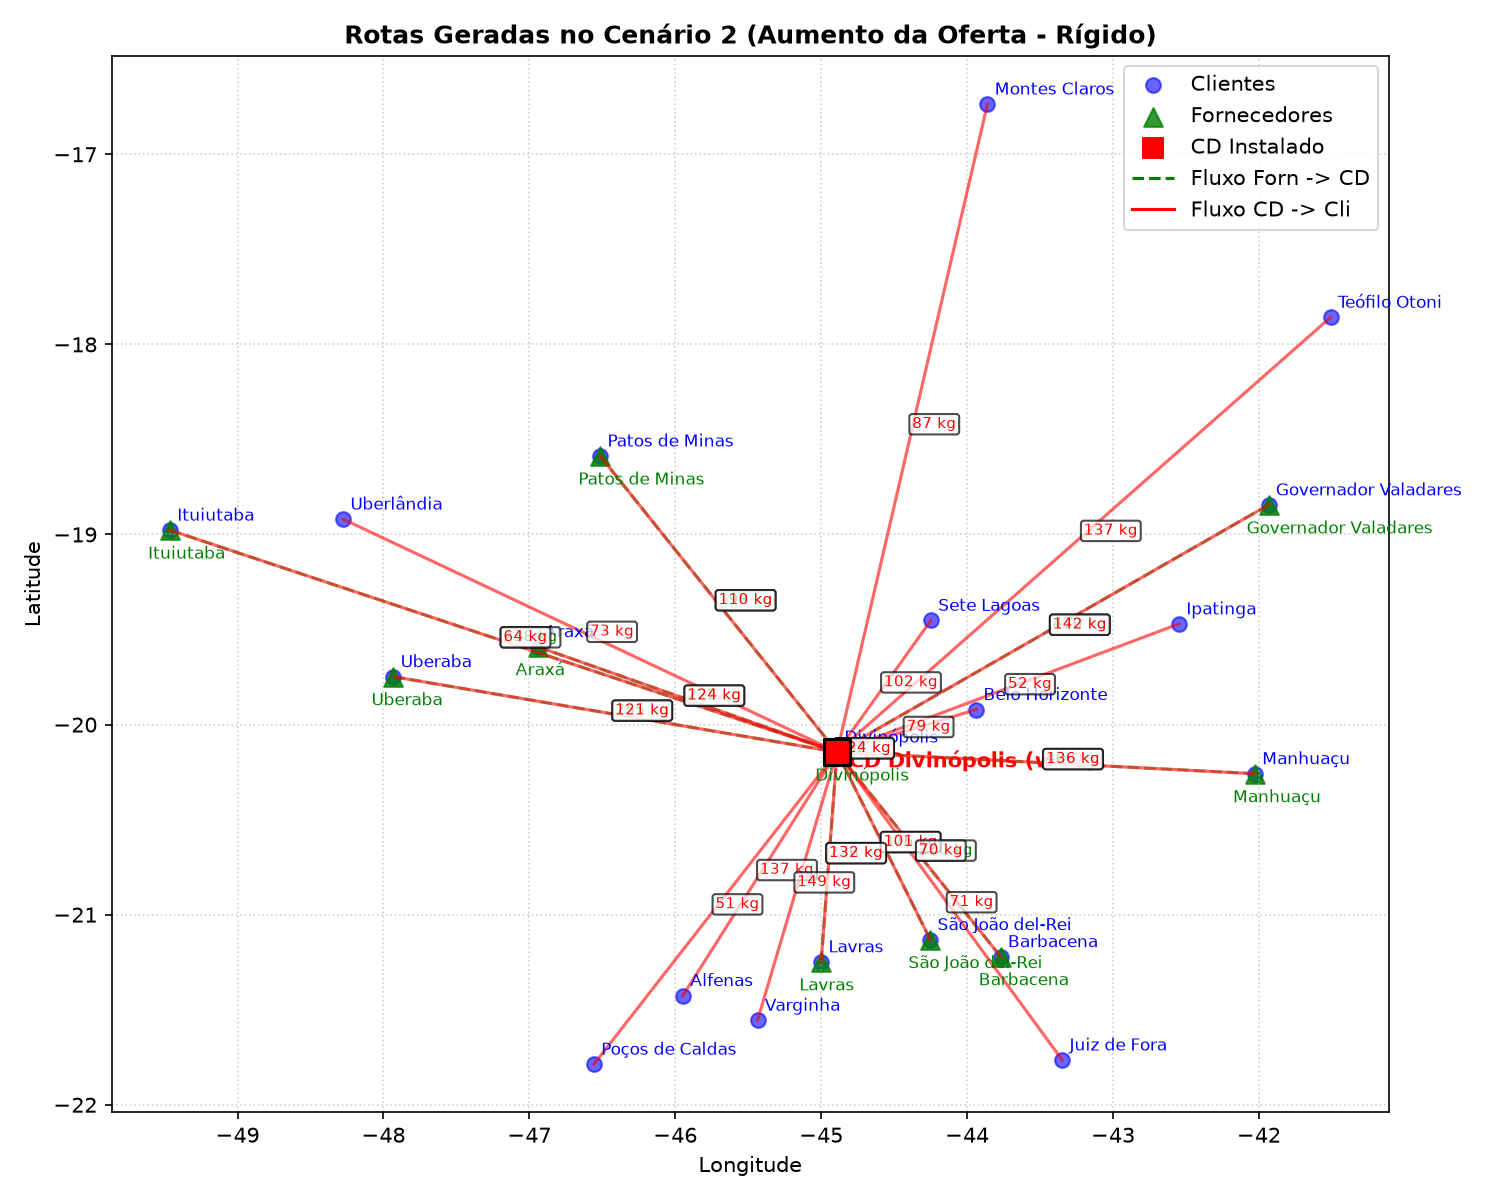
\includegraphics[width=0.95\textwidth]{imgs/mapa_cenario_2.png}
\caption{Rotas geradas no Cenário 2 centralizadas em Divinópolis}
\label{fig:mapa_cenario_2}
\end{figure}

% =========================================
\section{Cenário Extra 2 - Flexibilização de Abastecimento}
% =========================================

Como forma de explorar a sensibilidade do modelo e analisar possíveis soluções para o elevado custo de estoque gerado pelo Cenário 2, propõe-se um cenário extra com uma mudança estrutural na modelagem. No modelo original, a restrição (3) força o recolhimento e processamento de toda a oferta disponível dos fornecedores:
\[
\sum_{k \in K} x_{ik} = s_i \quad \forall i \in I
\]
No entanto, na prática de cadeias de suprimentos, uma empresa não precisa comprar obrigatoriamente toda a oferta se ela excede as demandas do mercado consumidor. Assim, nesta proposta extra, a restrição (3) é relaxada para uma desigualdade (transformando-se em redundante frente à restrição 2), de modo que o recolhimento de matéria-prima passe a ser opcional:
\[
\sum_{k \in K} x_{ik} \le s_i \quad \forall i \in I
\]

A Tabela \ref{tab:cenario2_extra_custos} apresenta os resultados financeiros sob essa modelagem flexível. Nota-se que o custo total cai de R\$ 131.135,96 para R\$ 19.592,43, representando uma economia drástica e eliminando totalmente o estoque residual e sua respectiva penalidade.

\begin{table}[H]
\centering
\begin{tabular}{lccc}
\hline
\textbf{Componente de Custo} & \textbf{Valor (R\$)} & \textbf{Representatividade (\%)} \\ \hline
Custo Total             & 19592,43  & 100\%     \\
Processamento (Torr)    & 12784,40  & $\sim$65,3\%  \\
Instalação de CDs       &  6000,00  & $\sim$30,6\%  \\
Transporte CD->Cli      &   488,43  & $\sim$2,5\%  \\
Transporte Forn->CD     &   319,60  & $\sim$1,6\%  \\
Penalidade de Estoque   &     0,00  & $\sim$0,0\%    \\
\hline
\end{tabular}
\caption{Resultados Financeiros do Cenário Extra 2}
\label{tab:cenario2_extra_custos}
\end{table}

\subsection{Efeito de Sourcing Estratégico}

Ao desobrigar a compra do excesso de café, o total processado cai de 3093,00 kg para a demanda exata dos clientes de 2062,00 kg. Com isso, os CDs não precisam mais das torrefadoras de maior capacidade. O solver abre o CD em Divinópolis ($w_{Divinopolis} = 2,0$), mas agora aloca as torrefadoras T1 (a mais barata de todas) e T2. A capacidade combinada de T1 e T2 ($1458 + 1580 = 3038$ kg) é suficiente para processar os 2062,00 kg, barateando o processamento para R\$ 12.784,40.

Mais do que isso, a maior oferta no mercado gera um forte efeito de otimização de sourcing (compras). Como o solver tem um "cardápio" maior de oferta disponível, ele pode escolher comprar preferencialmente dos fornecedores mais próximos de Divinópolis, deixando de adquirir café dos fornecedores geograficamente distantes (Ituiutaba, Uberaba e Governador Valadares).

Esse aproveitamento se reflete diretamente no custo de transporte inbound (Fornecedor $\rightarrow$ CD): enquanto no cenário base (onde a oferta era menor e rígida) o custo de transporte de fornecedores para os CDs era de R\$ 654,57, no cenário extra com oferta flexível esse custo desaba para apenas R\$ 319,60 (queda de 51,2\%).

A Tabela \ref{tab:cenario2_extra_forn_cd} apresenta como o fluxo se concentrou apenas nos fornecedores locais e vizinhos a Divinópolis. O total de viagens inbound cai de 10 viagens para apenas 7 viagens.

\begin{table}[H]
\centering
\begin{tabular}{llcc}
\hline
\textbf{Origem (Fornecedor)} & \textbf{Destino (CD)} & \textbf{Quantidade (kg)} & \textbf{Viagens} \\ \hline
São João del-Rei & Divinópolis & 376,50 & 1 \\
Patos de Minas & Divinópolis & 198,00 & 1 \\
Barbacena & Divinópolis & 259,50 & 1 \\
Lavras & Divinópolis & 235,50 & 1 \\
Manhuaçu & Divinópolis & 338,50 & 1 \\
Divinópolis & Divinópolis & 432,00 & 1 \\
Araxá & Divinópolis & 222,00 & 1 \\
Governador Valadares & Divinópolis & 0,00 & 0 \\
Ituiutaba & Divinópolis & 0,00 & 0 \\
Uberaba & Divinópolis & 0,00 & 0 \\ \hline
\textbf{Total} & & \textbf{2062,00} & \textbf{7} \\
\hline
\end{tabular}
\caption{Distribuição dos fornecedores para os CDs no Cenário Extra 2}
\label{tab:cenario2_extra_forn_cd}
\end{table}

A Figura \ref{fig:mapa_cenario_2_extra} mostra as rotas otimizadas resultantes do Cenário Extra 2, nas quais os fornecedores do Triângulo Mineiro e do Leste do estado (Governador Valadares) são excluídos do fluxo logístico, resultando em uma malha mais compacta e econômica.

\begin{figure}[H]
\centering
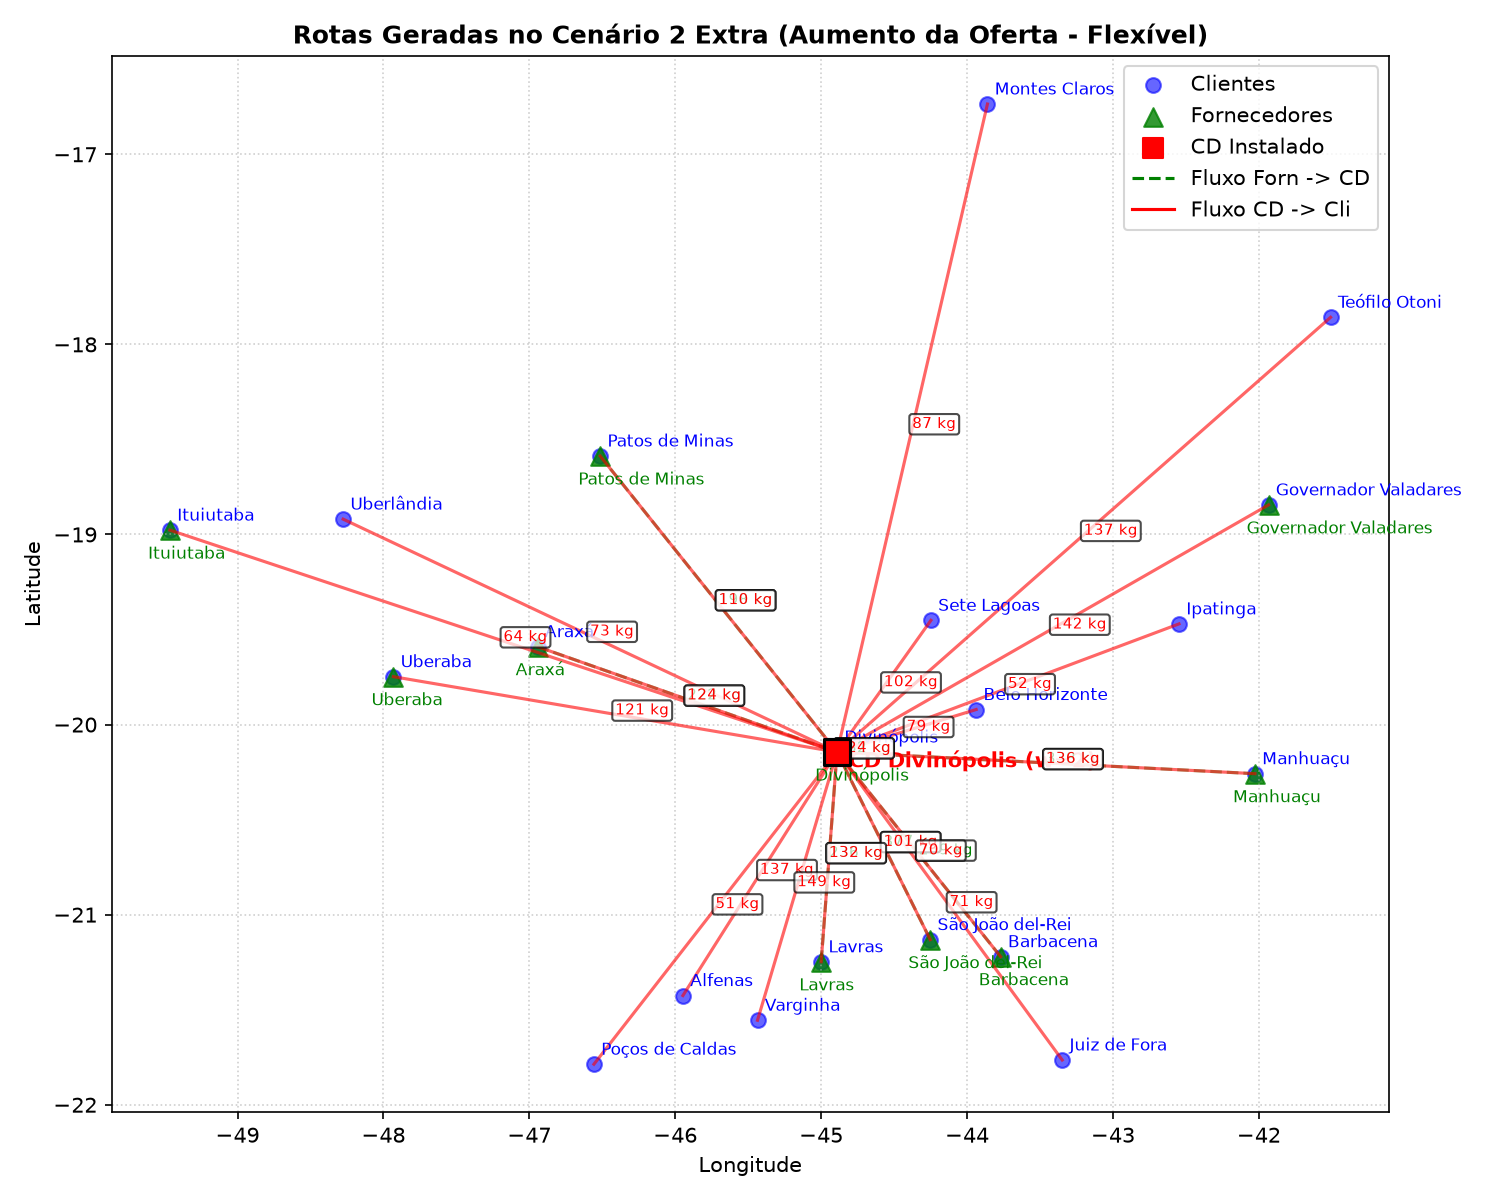
\includegraphics[width=0.95\textwidth]{imgs/mapa_cenario_2_extra.png}
\caption{Rotas geradas no Cenário Extra 2 com seleção otimizada de fornecedores}
\label{fig:mapa_cenario_2_extra}
\end{figure}

% =========================================
\section{Cenário 3}
% =========================================


O cenário 3 é focado no aumento da demanda dos clientes, em particular num aumento em 30\%. Neste cenário, entretanto, a demanda total supera a oferta total. Então, ao tentar executar o programa, um erro foi obtido, pois não havia solução viável para aquela instância. A instância em particular possuía os seguintes valores:

\begin{table}[h]
\centering
\begin{tabular}{lccc}
\hline
\textbf{Cidade} & \textbf{lat} & \textbf{lon} & \textbf{oferta} \\ \hline
São João del-Rei & -21.1314 & -44.2526 & 297.6358 \\
Governador Valadares & -18.8443 & -41.9339 & 371.1554 \\
Ituiutaba & -18.9772 & -49.4632 & 188.5422 \\
Uberaba & -19.748 & -47.9319 & 201.586 \\
Patos de Minas & -18.5873 & -46.5146 & 156.5256 \\
Barbacena & -21.221 & -43.77 & 205.1434 \\
Lavras & -21.248 & -45 & 186.1706 \\
Manhuaçu & -20.2584 & -42.0274 & 321.3518 \\
Divinópolis & -20.1446 & -44.8912 & 341.5104 \\
Araxá & -19.5902 & -46.9438 & 175.4984 \\ 
\textbf{Total} & & & 2245.1196 \\
\hline
\end{tabular}
\caption{Cidades e ofertas}
\label{tab:dados_cidades}
\end{table}

\begin{table}[ht]
\centering
\begin{tabular}{lrrr}
\hline
\textbf{Cidade} & \textbf{lat} & \textbf{lon} & \textbf{demanda} \\
\hline
São João del-Rei & -21.1314 & -44.2526 & 196.95 \\
Governador Valadares & -18.8443 & -41.9339 & 276.9 \\
Ituiutaba & -18.9772 & -49.4632 & 124.8 \\
Uberaba & -19.748 & -47.9319 & 235.95 \\
Patos de Minas & -18.5873 & -46.5146 & 214.5 \\
Barbacena & -21.221 & -43.77 & 91 \\
Lavras & -21.248 & -45 & 171.6 \\
Manhuaçu & -20.2584 & -42.0274 & 176.8 \\
Divinópolis & -20.1446 & -44.8912 & 161.2 \\
Araxá & -19.5902 & -46.9438 & 161.2 \\
Alfenas & -21.4256 & -45.9477 & 178.1 \\
Varginha & -21.5556 & -45.4364 & 193.7 \\
Uberlândia & -18.9192 & -48.2764 & 94.9 \\
Ipatinga & -19.4703 & -42.5476 & 67.6 \\
Juiz de Fora & -21.7645 & -43.3481 & 92.3 \\
Sete Lagoas & -19.4516 & -44.2479 & 132.6 \\
Poços de Caldas & -21.7868 & -46.5576 & 66.3 \\
Teófilo Otoni & -17.8574 & -41.5086 & 178.1 \\
Belo Horizonte & -19.9208 & -43.9378 & 102.7 \\
Montes Claros & -16.7354 & -43.8604 & 113.1 \\
\textbf{Total} & & & 3030.3 \\
\hline
\end{tabular}
\caption{Cidades e demandas}
\label{tab:dados_cidades}
\end{table}

\newpage
Observa-se que a demanda total dos clientes, isto é, a soma das demandas de cada cliente, vale 3030.3, enquanto a oferta total dos fornecedores vale 2245.1196. Ao inspecionar as restrições do modelo, o motivo para que a instância falhe está nas seguintes restrições:

\[
(3) \; \; \sum_{k \in K} x_{ik} = s_i \; \; \; \forall i \in I
\]

Que garante que toda a oferta seja utilizada e,

\[
(4) \; \; \sum_{k \in K} y_{kj} \geq d_j \; \; \; \forall j \in J
\]

\[
(5) \; \; \sum_{k \in K} y_{kj} \leq d_j \; \; \; \forall j \in J
\]

Que garantem que toda a demanda seja atendida. 

É impossível que todas as restrições sejam atendidas em um cenário onde a demanda seja maior que a oferta, pois falta produto para ser enviado para os clientes. Ou seja, a empresa não consegue lidar com um salto de 30\% da demanda imposta pelos seus clientes, sendo necessário aumentar a oferta dos fornecedores para atender essa demanda proposta.

% =========================================
\section{Cenário 4 - Custo Fixo Diferenciado}
% =========================================

O Cenário 4 explora a sensibilidade da rede logística a variações nos custos fixos de instalação dos Centros de Distribuição (CDs). Diferente de instâncias onde há inviabilidade por desbalanço insustentável entre oferta e demanda, este cenário obteve uma solução viável. O objetivo desta etapa é avaliar os efeitos dos parâmetros na cadeia[cite: 4], notando-se que as decisões operacionais do modelo focaram na centralização extrema do fluxo logístico.

A tabela abaixo detalha os resultados financeiros da operação, evidenciando que os custos de processamento e a penalidade de estoque representam, juntos, quase 80\% do gasto total, enquanto o transporte possui um impacto financeiro marginal.

\begin{table}[H]
\centering
\begin{tabular}{lccc}
\hline
\textbf{Componente de Custo} & \textbf{Valor (R\$)} & \textbf{Representatividade (\%)} \\ \hline
Custo Total             & 33693,48  & 100\%     \\
Processamento (Torr)    & 15159,74  & ~45,0\%  \\
Penalidade de Estoque   & 11411,96  & ~33,9\%  \\
Instalação de CDs       &  6000,00  & ~17,8\%  \\
Transporte CD->Cli      &   567,84  & ~1,7\%  \\
Transporte Forn->CD     &   553,94  & ~1,6\%    \\
\hline
\end{tabular}
\caption{Resultados Financeiros do Cenário 4}
\label{tab:cenario4_custos}
\end{table}

Ao analisar a infraestrutura escolhida, constata-se a abertura de apenas um único Centro de Distribuição, localizado em Divinópolis ($w_{Divinopolis} = 1$). Para dar vazão ao volume, foram utilizadas as torrefadoras locais T1 e T2 associadas a este CD ($z_{Divinopolis, T1} = 1$ e $z_{Divinopolis, T2} = 1$). 

Enquanto, a tabela \ref{tab:cenario4_forn_cd} demonstra como a oferta de entrada (inbound) dos dez fornecedores do estado foi integralmente direcionada a esse único polo.

\begin{table}[H]
\centering
\begin{tabular}{lccc}
\hline
\textbf{Origem (Fornecedor)} & \textbf{Destino (CD)} & \textbf{Quantidade} \\ \hline
São João del-Rei        & CD Divinópolis    & 297,64 kg     \\
Governador Valadares    & CD Divinópolis    & 371,16 kg  \\
Ituiutaba               & CD Divinópolis    & 188,54 kg  \\
Uberaba                 & CD Divinópolis    & 201,59 kg  \\
Patos de Minas          & CD Divinópolis    & 156,53 kg  \\
Barbacena               & CD Divinópolis    & 205,14 kg \\
Lavras                  & CD Divinópolis    & 186,17 kg \\
Manhuaçu                & CD Divinópolis    & 321,35 kg  \\
Divinópolis             & CD Divinópolis    & 341,51 kg  \\
Araxá                   & CD Divinópolis    & 175,50 kg  \\
\hline
\end{tabular}
\caption{Distribuição de Fornecedores para CDs}
\label{tab:cenario4_forn_cd}
\end{table}

De forma análoga, a Tabela \ref{tab:cenario4_cd_cli} ilustra a etapa de escoamento (outbound). Nela, observa-se o CD de Divinópolis operando como o nó exclusivo de distribuição para atender à demanda de todas as vinte cidades clientes.

\begin{table}[H]
\centering
\begin{tabular}{llc}
\hline
\textbf{Origem (CD)} & \textbf{Destino (Cliente)} & \textbf{Quantidade} \\ \hline
CD Divinópolis  & São João del-Rei          & 151,50 kg     \\
CD Divinópolis  & Governador Valadares      & 213,00 kg     \\
CD Divinópolis  & Ituiutaba                 &  96,00 kg    \\
CD Divinópolis  & Uberaba                   & 181,50 kg     \\
CD Divinópolis  & Patos de Minas            & 165,00 kg     \\
CD Divinópolis  & Barbacena                 &  70,00 kg    \\
CD Divinópolis  & Lavras                    & 132,00 kg     \\
CD Divinópolis  & Manhuaçu                  & 136,00 kg     \\
CD Divinópolis  & Divinópolis               & 124,00 kg     \\
CD Divinópolis  & Araxá                     & 124,00 kg     \\
CD Divinópolis  & Alfenas                   & 137,00 kg     \\
CD Divinópolis  & Varginha                  & 149,00 kg     \\
CD Divinópolis  & Uberlândia                &  73,00 kg    \\
CD Divinópolis  & Ipatinga                  &  52,00 kg    \\
CD Divinópolis  & Juiz de Fora              &  71,00 kg    \\
CD Divinópolis  & Sete Lagoas               & 102,00 kg     \\
CD Divinópolis  & Poços de Caldas           &  51,00 kg    \\
CD Divinópolis  & Teófilo Otoni             & 137,00 kg     \\
CD Divinópolis  & Belo Horizonte            &  79,00 kg    \\
CD Divinópolis  & Montes Claros             &  87,00 kg    \\
\hline
\end{tabular}
\caption{Distribuição de CDs para clientes}
\label{tab:cenario4_cd_cli}
\end{table}

A visualização geográfica e o impacto visual da escolha por um único CD podem ser observados na Figura \ref{fig:mapa_cenario_4}, que consolida a malha rodoviária gerada no cenário.

\begin{figure}[H]
\centering
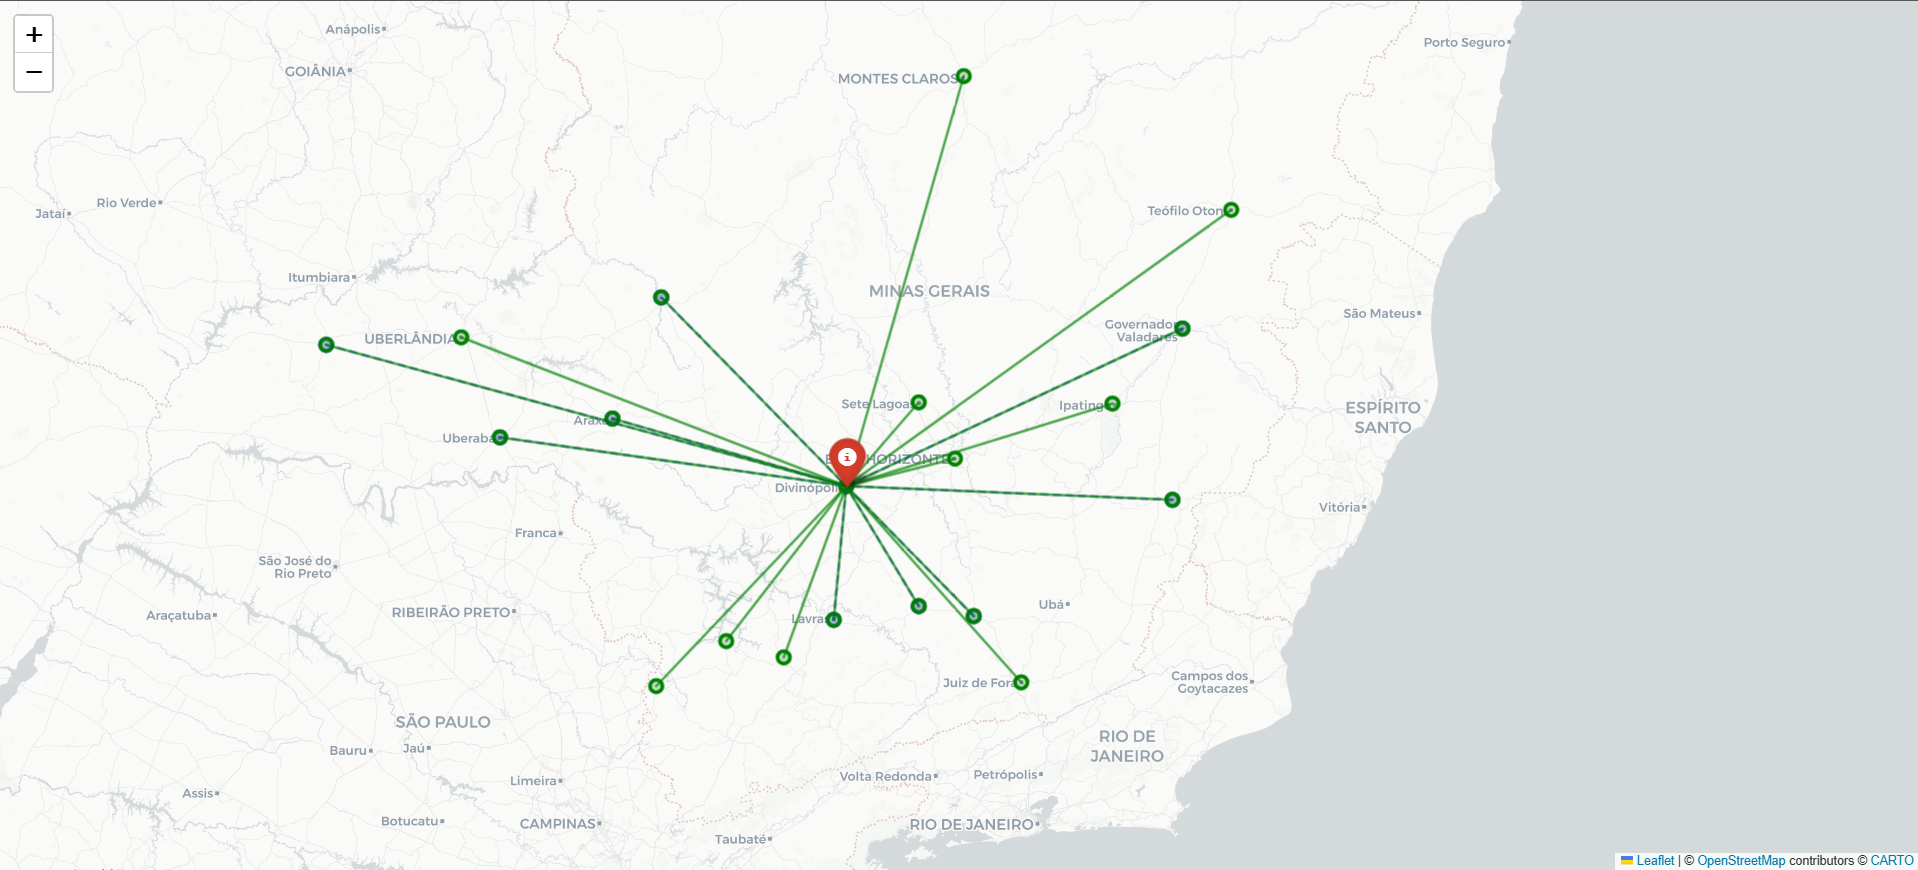
\includegraphics[width=0.95\textwidth]{imgs/mapa_cenario_4.png}
\caption{Rotas geradas no cenário 4 centralizadas em Divinópolis}
\label{fig:mapa_cenario_4}
\end{figure}

\subsection{Comportamento Matemático e Trade-offs Logísticos}

O comportamento centralizador do modelo é uma resposta direta à sua Função Objetivo, que busca minimizar os custos totais:

$$\min \sum_{i\in I}\sum_{k\in K}c_{ik}x_{ik}+\sum_{k\in K}\sum_{j\in J}c_{kj}y_{kj}+\sum_{k\in K}f_{k}w_{k}+\sum_{i\in I}\sum_{k\in K}\sum_{t\in T}p_{t}u_{ikt}+\sum_{k\in K}pen\cdot e_{k}$$

Com a alteração dos custos fixos no Cenário 4, o parâmetro $f_k$ dos outros CDs candidatos se tornou muito elevado em relação a Divinópolis. O modelo matemático calculou que a economia obtida nas distâncias de transporte ao abrir mais de um CD não seria suficiente para compensar o pagamento de um novo custo de instalação $f_k$. De fato, os custos totais de transporte (Fornecedor $\rightarrow$ CD e CD $\rightarrow$ Cliente) representam, juntos, apenas cerca de 3,3\% dos gastos totais. Assim, consolidar o fluxo no CD de Divinópolis (cujo $f_k = 6000$) revelou-se a decisão mais econômica. 

Outro impacto significativo revelado pela solução é o alto custo de retenção, guiado pela restrição de conservação de fluxo da equação 6:  

$$\sum_{i\in I}x_{ik}=\sum_{j\in J}y_{kj}+e_{k} \;\;\; \forall k\in K$$

Por meio das restrições (2) e (3), o modelo é obrigado a escoar toda a oferta disponível $s_i$. Somando as remessas dos 10 fornecedores, o total enviado a Divinópolis ($\sum x_{ik}$) é de aproximadamente 2.245,13 kg. Paralelamente, as restrições (4) e (5) garantem que os envios aos clientes ($\sum y_{kj}$) igualem rigidamente suas demandas exatas $d_j$, totalizando 2.131,00 kg.

Substituindo esses valores na Equação 6, observamos que a diferença entre a entrada compulsória e a saída limitada obriga a geração de um estoque residual $e_k$: 

$$2245,13 = 2131,00 + e_{Divinopolis} \implies e_{Divinopolis} \approx 114,13 \text{ kg}$$

Como a penalidade predefinida ($pen$) é de 100 por unidade processada, justifica-se matematicamente a penalidade total apresentada: $114,13 \text{ kg} \times 100 \approx \text{R\$} 11.413,00$ (com pequenas variações por arredondamento fracionário nos totais reais calculados de R\$ 11.411,96). Conclui-se que o gargalo da rede atual não reside no transporte logístico, mas no custo imposto pela absorção de uma oferta sistêmica superior à demanda do mercado.

\section{Cenário extra - Torrefadora indisponível}

O cenário seguinte explora a indisponibilidade de uma das três torrefadoras utilizadas no cenário base. Isto é, foram consideradas apenas as torrefadoras T2 e T3 com o restante dos parâmetros invariante. O mapa gerado após a execução do cenário é: 

\begin{figure}[h]
    \centering
    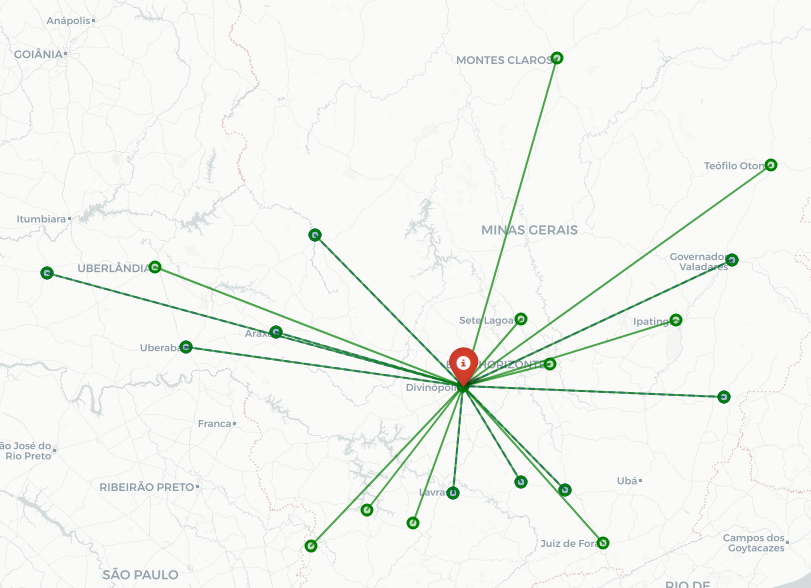
\includegraphics[width=0.5\textwidth]{imgs/mapa_cenario_extra.png}
    \caption{Mapa das rotas geradas no cenário extra}
    \label{fig:cruzeiro}
\end{figure} 

O mapa nestas condições se mostrou bastante alterado em relação ao mapa obtido no Cenário 1, com apenas um CD construído, ao contrário dos dois CDs do primeiro cenário. Isso está diretamente ligado à capacidade que a torrefadora T1 proporcionava, conforme a tabela abaixo: 

\begin{table}[h] 
\centering

\label{tab:torrefadoras}
\begin{tabular}{lccc}
\hline
\textbf{Torrefadora} & \textbf{Capacidade} & \textbf{Custo de processamento} & \textbf{Tempo de processamento} \\
\hline
T1 & 1458 & 6.20 & 1.40 \\
T2 & 1580 & 6.74 & 2.03 \\
T3 & 1587 & 8.71 & 2.18 \\
\hline
\end{tabular}
\caption{Dados das torrefadoras originais}
\end{table} 

A torrefadora T1 era a mais barata e a mais rápida, sendo assim sua interrupção causou impacto na operação e topologia de transporte. Em particular, para minimizar o custo total, o modelo verificou que o custo de construir um novo CD superava o custo de transporte de rotas mais longas, e então abriu mão de construir o segundo CD, deixando a operação totalmente centralizada em uma única instalação, com duas torrefadoras atreladas a essa localidade. O resultado dessa mudança foi um aumento no custo total:

\begin{table}[h]
\centering

\label{tab:resultados_financeiros}
\begin{tabular}{lr}
\hline
\textbf{Item} & \textbf{Valor (R\$)} \\
\hline
Transporte Fornecedor $\rightarrow$ CD & 934.28 \\
Transporte CD $\rightarrow$ Clientes & 976.86 \\
Instalação de CDs & 6000.00 \\
Processamento (Torrefadoras) & 13897.88 \\
Penalidade de Estoque & 0.00 \\
\hline
\textbf{Custo Total} & \textbf{21809.02} \\
\hline
\end{tabular}

\caption{Resultados financeiros sem a torrefadora T1}
\end{table}

\newpage
Portanto, a realocação da topologia da empresa após a desativação da torrefadora não foi suficiente para manter o custo, havendo um aumento no custo total, associado majoritariamente ao processamento pelas torrefadoras e do transporte do CD ao cliente, que agora foi aumentado graças ao aumento do tamanho das rotas causado pela centraliação da operação.

% =========================================
\section{Cenário Extra - Resiliência e Expansão Modular da Infraestrutura}
% =========================================

Considerando o Cenário 4, como forma de aprofundar a análise de sensibilidade e propor novas discussões logísticas, propõe-se um cenário extra focado na resiliência da infraestrutura. A manipulação ocorreu diretamente nos dados de entrada, onde simulou-se uma falha de maquinário localizada: a capacidade das torrefadoras T1 e T2 foi reduzida para apenas 600 kg cada.

A Tabela \ref{tab:cenario_extra_custos} apresenta os novos custos da operação sob esta condição de estresse operacional.

\begin{table}[H]
\centering
\begin{tabular}{lccc}
\hline
\textbf{Componente de Custo} & \textbf{Valor (R\$)} & \textbf{Representatividade (\%)} \\ \hline
Custo Total             & 36693,48  & 100\%     \\
Processamento (Torr)    & 15159,74  & $\sim$41,3\%  \\
Penalidade de Estoque   & 11411,96  & $\sim$31,1\%  \\
Instalação de CDs       &  9000,00  & $\sim$24,5\%  \\
Transporte CD->Cli      &   567,84  & $\sim$1,5\%  \\
Transporte Forn->CD     &   553,94  & $\sim$1,5\%    \\
\hline
\end{tabular}
\caption{Resultados Financeiros do Cenário Extra}
\label{tab:cenario_extra_custos}
\end{table}

Ao aplicar a restrição nas torrefadoras ativas de Divinópolis, esperava-se que a saturação da restrição limitante forçasse o modelo a descentralizar a operação para outras cidades:

$$\sum_{i\in I}x_{ik}\le\sum_{t\in T}q_{t}z_{kt} \;\;\; \forall k\in K$$

No entanto, a malha de distribuição e as rotas permaneceram estáticas e centralizadas (conforme a Figura \ref{fig:mapa_cenario_extra_falha}), revelando uma característica comportamental da implementação computacional. Na codificação do algoritmo, a variável de decisão de instalação do CD ($w_k$) operou sem o limitante estrito de $w_k \le 1$. Diante do estrangulamento da capacidade, o solver optou por uma "expansão modular" no próprio polo de Divinópolis, elevando o valor de $w_k$ e incorrendo em um custo de instalação adicional de R\$ 3.000,00, totalizando assim R\$ 9.000,00. 

Essa decisão permitiu a ativação de uma terceira máquina (a torrefadora T3) no mesmo nó logístico. Conclui-se que o custo variável de transporte rodoviário na rede é tão insignificante que é financeiramente mais viável para a empresa expandir a infraestrutura física de um mesmo polo (mesmo pagando novos custos fixos repetidamente) do que arcar com as despesas logísticas de escoamento para a abertura de um novo Centro de Distribuição em outra cidade.

\begin{figure}[H]
\centering
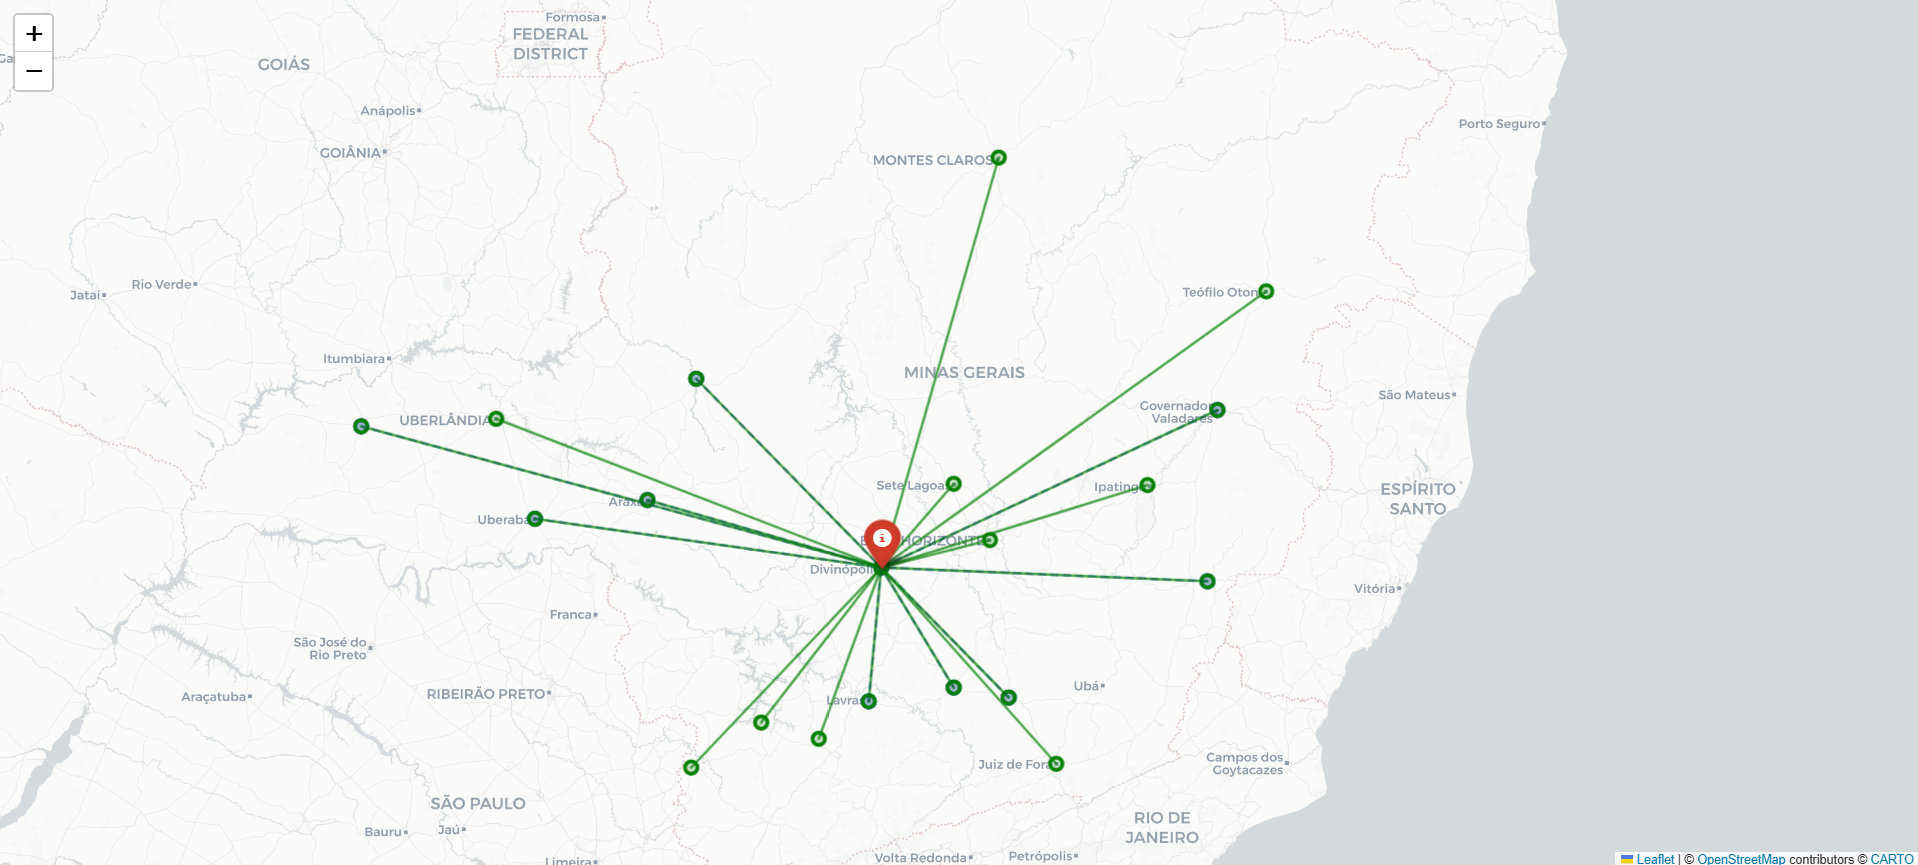
\includegraphics[width=0.95\textwidth]{imgs/mapa_cenario_extra_falha_localizada.png}
\caption{Manutenção da malha centralizada em Divinópolis através da expansão modular}
\label{fig:mapa_cenario_extra_falha}
\end{figure}

\section{Cenário 5 - Capacidade reduzida dos caminhões}

\subsection{Modelagem do problema}

O Cenário 5 e o cenário extra foram modelados a partir da mesma estrutura de otimização utilizada no cenário base. O problema considera fornecedores, candidatos a centros de distribuição, clientes e torrefadoras. A decisão do modelo consiste em definir quais centros de distribuição serão abertos, quais torrefadoras serão alocadas a esses centros e quais fluxos de café devem ocorrer entre fornecedores, CDs e clientes, buscando minimizar o custo total da operação.

Sejam $I$ o conjunto de fornecedores, $J$ o conjunto de clientes, $K$ o conjunto de candidatos a centros de distribuição e $T$ o conjunto de torrefadoras. As principais variáveis de decisão são: $x_{ik}$, quantidade enviada do fornecedor $i$ para o CD $k$; $y_{kj}$, quantidade enviada do CD $k$ para o cliente $j$; $w_k$, variável binária que indica se o CD $k$ será aberto; $z_{kt}$, variável binária que indica se a torrefadora $t$ será alocada ao CD $k$; $u_{ikt}$, quantidade processada pela torrefadora $t$; e $e_k$, estoque residual no CD $k$.

A função objetivo busca minimizar o custo total da rede logística:

\begin{equation*}
\min
\sum_{i \in I}\sum_{k \in K} c_{ik}x_{ik}
+
\sum_{k \in K}\sum_{j \in J} c_{kj}y_{kj}
+
\sum_{k \in K} f_kw_k
+
\sum_{i \in I}\sum_{k \in K}\sum_{t \in T} p_tu_{ikt}
+
\sum_{k \in K} pen \cdot e_k
\end{equation*}

em que $c_{ik}$ representa o custo de transporte entre fornecedores e CDs, $c_{kj}$ representa o custo de transporte entre CDs e clientes, $f_k$ representa o custo fixo de instalação do CD, $p_t$ representa o custo de processamento da torrefadora e $pen$ representa a penalidade por estoque residual.

As principais restrições garantem que toda a oferta seja enviada aos centros de distribuição:

\begin{equation*}
\sum_{k \in K} x_{ik} = s_i, \quad \forall i \in I
\end{equation*}

que toda a demanda dos clientes seja atendida:

\begin{equation*}
\sum_{k \in K} y_{kj} = d_j, \quad \forall j \in J
\end{equation*}

e que haja conservação de fluxo em cada centro de distribuição:

\begin{equation*}
\sum_{i \in I} x_{ik} =
\sum_{j \in J} y_{kj} + e_k,
\quad \forall k \in K
\end{equation*}

A alocação de torrefadoras depende da abertura dos CDs:

\begin{equation*}
\sum_{t \in T} z_{kt} \leq w_k,
\quad \forall k \in K
\end{equation*}

e a capacidade das torrefadoras alocadas deve ser suficiente para processar o volume recebido:

\begin{equation*}
\sum_{i \in I} x_{ik}
\leq
\sum_{t \in T} q_tz_{kt},
\quad \forall k \in K
\end{equation*}

Também foi mantido o limite máximo de centros de distribuição abertos:

\begin{equation*}
\sum_{k \in K} w_k \leq m
\end{equation*}

No Cenário 5, a principal alteração em relação ao cenário base foi a redução da capacidade dos caminhões para 300 kg. Como o custo de transporte é calculado com base na razão entre distância e capacidade do caminhão, essa mudança aumenta o custo unitário de deslocamento e permite avaliar o impacto da limitação de transporte na rede logística.

No cenário extra, foi mantida a mesma modelagem, mas com uma condição mais restritiva: a capacidade dos caminhões foi reduzida para 80 kg e os custos de instalação dos CDs de Araxá e Belo Horizonte foram elevados para R\$ 20.000,00. Com isso, o modelo passou a avaliar não apenas o impacto de veículos menores, mas também o efeito do encarecimento dos centros que haviam sido escolhidos no Cenário 5.
\subsection{ Problema Base}
O Cenário 5 avalia o impacto da redução da capacidade dos caminhões para 300 kg. Em relação ao cenário base, os demais parâmetros foram mantidos, permitindo observar especificamente como a limitação de transporte influencia os custos, as rotas e a operação logística. No código utilizado, o custo de transporte entre dois pontos é calculado pela razão entre a distância geográfica e a capacidade do caminhão. Assim, ao reduzir a capacidade, o custo unitário de transporte aumenta, mesmo quando a estrutura geral das rotas permanece parecida.

Após a execução do modelo, foi encontrada uma solução viável com custo total de \textbf{R\$ 21.427,59}. A decomposição dos custos é apresentada na Tabela \ref{tab:cenario5_custos}.

\begin{table}[htbp]
\centering
\small
\begin{tabular}{lr}
\hline
\textbf{Componente de custo} & \textbf{Valor (R\$)} \\ \hline
Transporte fornecedor--CD & 1.087,82 \\
Transporte CD--cliente & 1.226,51 \\
\textbf{Transporte total} & \textbf{2.314,33} \\
Instalação de CDs & 6.000,00 \\
Processamento nas torrefadoras & 13.113,26 \\
Estoque & 0,00 \\ \hline
\textbf{Custo total} & \textbf{21.427,59} \\ \hline
\end{tabular}
\caption{Componentes de custo no Cenário 5}
\label{tab:cenario5_custos}
\end{table}

Os centros de distribuição abertos foram \textbf{Araxá} e \textbf{Belo Horizonte}. O CD de Araxá utilizou a torrefadora \textbf{T2}, enquanto o CD de Belo Horizonte utilizou a torrefadora \textbf{T1}. Não houve estoque final nos CDs, indicando que toda a quantidade recebida foi encaminhada para atendimento da demanda dos clientes.

\begin{table}[htbp]
\centering
\small
\begin{tabular}{llrrr}
\hline
\textbf{CD aberto} & \textbf{Torrefadora} & \textbf{Entrada (kg)} & \textbf{Saída (kg)} & \textbf{Estoque (kg)} \\ \hline
Araxá & T2 & 609,00 & 609,00 & 0,00 \\
Belo Horizonte & T1 & 1.453,00 & 1.453,00 & 0,00 \\ \hline
\end{tabular}
\caption{CDs abertos, torrefadoras utilizadas e balanço de fluxo no Cenário 5}
\label{tab:cenario5_cds}
\end{table}

A Tabela \ref{tab:cenario5_fornecedor_cd} apresenta a distribuição dos fornecedores para os CDs. Para estimar o número de viagens, considerou-se o arredondamento para cima da razão entre a quantidade transportada em cada rota e a capacidade do caminhão de 300 kg.

{\footnotesize
\begin{longtable}{p{4.2cm}p{3.3cm}rr}
\caption{Distribuição dos fornecedores para os CDs no Cenário 5}\label{tab:cenario5_fornecedor_cd}\\
\hline
\textbf{Fornecedor} & \textbf{CD} & \textbf{Quantidade (kg)} & \textbf{Viagens} \\ \hline
\endfirsthead
\hline
\textbf{Fornecedor} & \textbf{CD} & \textbf{Quantidade (kg)} & \textbf{Viagens} \\ \hline
\endhead
São João del-Rei & Belo Horizonte & 251,00 & 1 \\
Governador Valadares & Belo Horizonte & 313,00 & 2 \\
Ituiutaba & Araxá & 159,00 & 1 \\
Uberaba & Araxá & 170,00 & 1 \\
Patos de Minas & Araxá & 132,00 & 1 \\
Barbacena & Belo Horizonte & 173,00 & 1 \\
Lavras & Belo Horizonte & 157,00 & 1 \\
Manhuaçu & Belo Horizonte & 271,00 & 1 \\
Divinópolis & Belo Horizonte & 288,00 & 1 \\
Araxá & Araxá & 148,00 & 1 \\ \hline
\end{longtable}
}

A Tabela \ref{tab:cenario5_cd_cliente} apresenta a distribuição dos CDs para os clientes.

{\footnotesize
\begin{longtable}{p{3.3cm}p{4.0cm}rr}
\caption{Distribuição dos CDs para os clientes no Cenário 5}\label{tab:cenario5_cd_cliente}\\
\hline
\textbf{CD} & \textbf{Cliente} & \textbf{Quantidade (kg)} & \textbf{Viagens} \\ \hline
\endfirsthead
\hline
\textbf{CD} & \textbf{Cliente} & \textbf{Quantidade (kg)} & \textbf{Viagens} \\ \hline
\endhead
Araxá & Ituiutaba & 64,00 & 1 \\
Araxá & Uberaba & 121,00 & 1 \\
Araxá & Patos de Minas & 110,00 & 1 \\
Araxá & Araxá & 124,00 & 1 \\
Araxá & Alfenas & 66,00 & 1 \\
Araxá & Uberlândia & 73,00 & 1 \\
Araxá & Poços de Caldas & 51,00 & 1 \\
Belo Horizonte & São João del-Rei & 101,00 & 1 \\
Belo Horizonte & Governador Valadares & 142,00 & 1 \\
Belo Horizonte & Barbacena & 70,00 & 1 \\
Belo Horizonte & Lavras & 132,00 & 1 \\
Belo Horizonte & Manhuaçu & 136,00 & 1 \\
Belo Horizonte & Divinópolis & 124,00 & 1 \\
Belo Horizonte & Alfenas & 71,00 & 1 \\
Belo Horizonte & Varginha & 149,00 & 1 \\
Belo Horizonte & Ipatinga & 52,00 & 1 \\
Belo Horizonte & Juiz de Fora & 71,00 & 1 \\
Belo Horizonte & Sete Lagoas & 102,00 & 1 \\
Belo Horizonte & Teófilo Otoni & 137,00 & 1 \\
Belo Horizonte & Belo Horizonte & 79,00 & 1 \\
Belo Horizonte & Montes Claros & 87,00 & 1 \\ \hline
\end{longtable}
}

No total, foram estimadas \textbf{11} viagens dos fornecedores para os CDs e \textbf{21} viagens dos CDs para os clientes, totalizando \textbf{32} viagens. Comparando com o cenário base, o número total estimado de viagens permaneceu igual, pois a redução da capacidade fez a rota Governador Valadares--Belo Horizonte passar a exigir duas viagens, mas a solução também eliminou uma rota pequena que existia no cenário base, de Patos de Minas para Belo Horizonte. Mesmo assim, o custo de transporte aumentou de R\$ 1.390,87 para R\$ 2.314,33, uma elevação de aproximadamente \textbf{66,39\%}.

\begin{figure}[htbp]
\centering
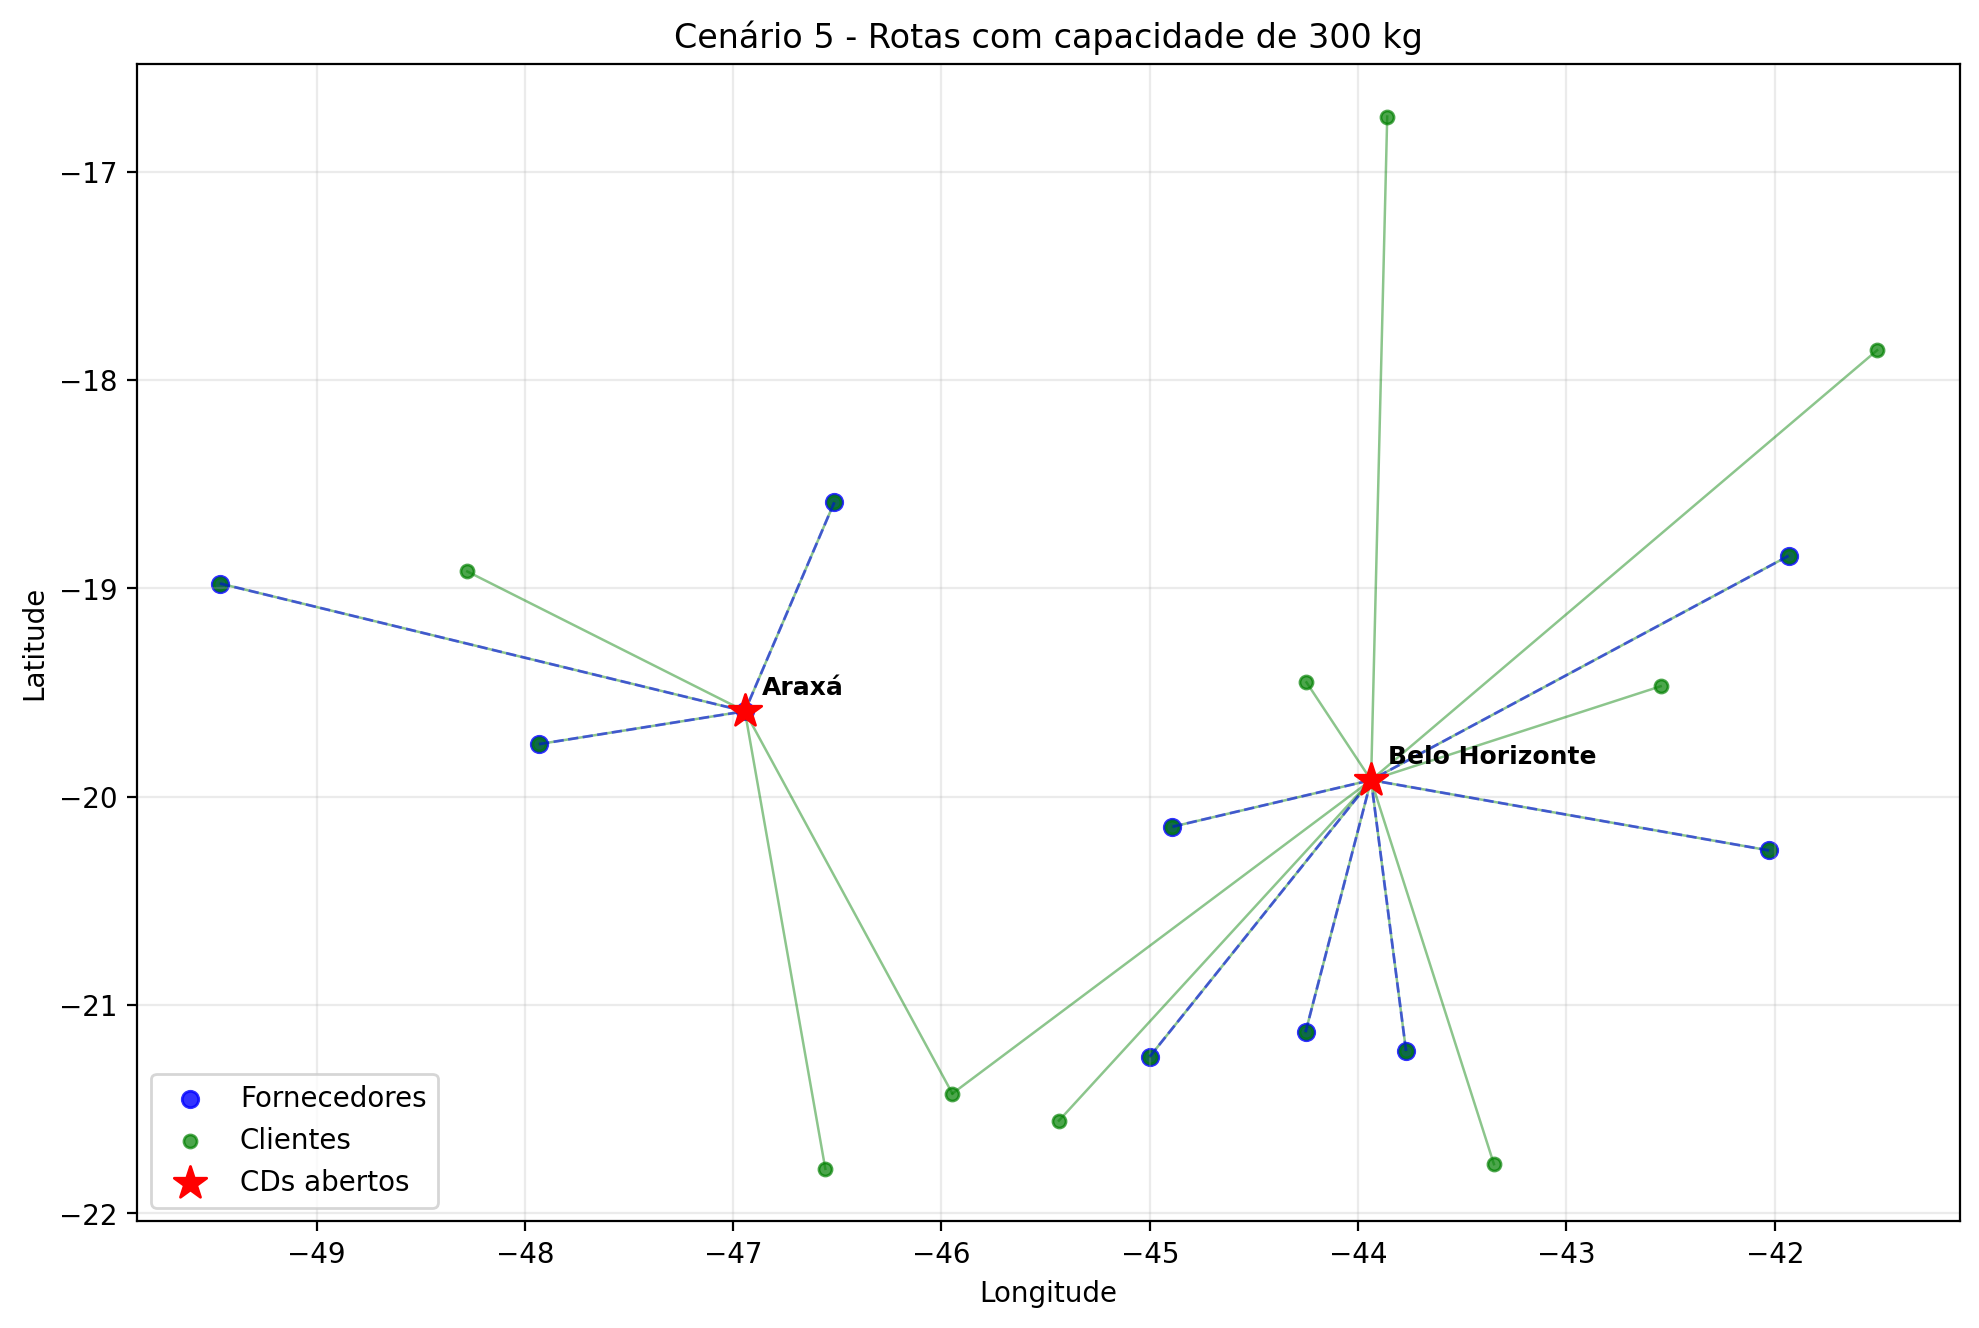
\includegraphics[draft=false,width=0.95\textwidth]{imgs/mapa_cenario5.png}
\caption{Rotas geradas no Cenário 5}
\label{fig:mapa_cenario5}
\end{figure}

A Figura \ref{fig:mapa_cenario5} apresenta o mapa das rotas geradas para o Cenário 5. As linhas tracejadas representam o fluxo dos fornecedores para os CDs, enquanto as linhas contínuas representam o fluxo dos CDs para os clientes.

De forma geral, a redução da capacidade dos caminhões tornou o transporte mais caro e aumentou a pressão operacional sobre a distribuição. A estrutura da solução permaneceu concentrada em dois CDs, Araxá e Belo Horizonte, mas o custo total subiu de R\$ 20.501,43 no cenário base para R\$ 21.427,59 no Cenário 5, um aumento de aproximadamente \textbf{4,52\%}. Esse resultado mostra que a capacidade dos veículos é um parâmetro relevante para a eficiência logística, pois influencia diretamente o custo de deslocamento e o aproveitamento das rotas.

% =========================================
\section{Cenário extra - Caminhões menores e CDs centrais com custo elevado}
% =========================================

Como cenário extra, foi construída uma situação mais restritiva do que a simples redução da capacidade dos caminhões. Nesse novo teste, a capacidade dos caminhões foi reduzida para 80 kg e os custos de instalação dos CDs de Araxá e Belo Horizonte foram elevados para R\$ 20.000,00. A ideia é simular um caso em que a empresa, além de operar com veículos menores, enfrenta restrições operacionais nos CDs que eram mais atrativos no Cenário 5, como aumento de aluguel, indisponibilidade temporária ou maior custo de implantação nesses locais.

A implementação desse cenário foi feita a partir da planilha do Cenário 5. Na aba de parâmetros, o valor da capacidade dos caminhões foi alterado para 80 kg. Além disso, na aba de candidatos a centros de distribuição, os custos de instalação de Araxá e Belo Horizonte foram alterados para R\$ 20.000,00. O restante dos dados foi mantido igual, de forma que a análise pudesse destacar o impacto conjunto da redução da capacidade de transporte e do encarecimento dos CDs anteriormente escolhidos.

Após a execução do modelo, foi encontrada uma solução viável com custo total de \textbf{R\$ 29.621,63}. A decomposição dos custos é apresentada na Tabela \ref{tab:cenario_extra_custos}.

\begin{table}[htbp]
\centering
\begin{tabular}{lr}
\hline
\textbf{Componente de custo} & \textbf{Valor (R\$)} \tabularnewline
\hline
Transporte fornecedor--CD & 4.935,15 \tabularnewline
Transporte CD--cliente & 5.526,78 \tabularnewline
Transporte total & 10.461,93 \tabularnewline
Instalação de CDs & 6.000,00 \tabularnewline
Processamento nas torrefadoras & 13.159,70 \tabularnewline
Estoque & 0,00 \tabularnewline
\hline
\textbf{Custo total} & \textbf{29.621,63} \tabularnewline
\hline
\end{tabular}
\caption{Componentes de custo no cenário extra}
\label{tab:cenario_extra_custos}
\end{table}

Diferentemente do Cenário 5, os centros de distribuição escolhidos foram \textbf{Barbacena} e \textbf{Divinópolis}. O CD de Barbacena utilizou a torrefadora \textbf{T2}, enquanto o CD de Divinópolis utilizou a torrefadora \textbf{T1}. Esse resultado mostra que o modelo deixou de escolher Araxá e Belo Horizonte quando esses centros passaram a ter custo de instalação elevado. Mesmo com o encarecimento desses dois CDs, o custo total de instalação permaneceu em R\$ 6.000,00, pois o modelo selecionou dois CDs alternativos com custo de instalação de R\$ 3.000,00 cada.

\begin{table}[htbp]
\centering
\begin{tabular}{llrrr}
\hline
\textbf{CD aberto} & \textbf{Torrefadora} & \textbf{Entrada (kg)} & \textbf{Saída (kg)} & \textbf{Estoque (kg)} \tabularnewline
\hline
Barbacena & T2 & 695,00 & 695,00 & 0,00 \tabularnewline
Divinópolis & T1 & 1.367,00 & 1.367,00 & 0,00 \tabularnewline
\hline
\end{tabular}
\caption{CDs abertos, torrefadoras utilizadas e balanço de fluxo no cenário extra}
\label{tab:cenario_extra_cds}
\end{table}

A Tabela \ref{tab:cenario_extra_fornecedor_cd} apresenta a distribuição dos fornecedores para os CDs no cenário extra. Para estimar o número de viagens, considerou-se o arredondamento para cima da razão entre a quantidade transportada na rota e a capacidade do caminhão de 80 kg.

\begin{longtable}{llrr}
\caption{Distribuição dos fornecedores para CDs no cenário extra}
\label{tab:cenario_extra_fornecedor_cd}\tabularnewline
\hline
\textbf{Fornecedor} & \textbf{CD} & \textbf{Quantidade (kg)} & \textbf{Viagens} \tabularnewline
\hline
\endfirsthead
\hline
\textbf{Fornecedor} & \textbf{CD} & \textbf{Quantidade (kg)} & \textbf{Viagens} \tabularnewline
\hline
\endhead
São João del-Rei & Barbacena & 251,00 & 4 \tabularnewline
Governador Valadares & Divinópolis & 313,00 & 4 \tabularnewline
Ituiutaba & Divinópolis & 159,00 & 2 \tabularnewline
Uberaba & Divinópolis & 170,00 & 3 \tabularnewline
Patos de Minas & Divinópolis & 132,00 & 2 \tabularnewline
Barbacena & Barbacena & 173,00 & 3 \tabularnewline
Lavras & Divinópolis & 157,00 & 2 \tabularnewline
Manhuaçu & Barbacena & 271,00 & 4 \tabularnewline
Divinópolis & Divinópolis & 288,00 & 4 \tabularnewline
Araxá & Divinópolis & 148,00 & 2 \tabularnewline
\hline
\end{longtable}

A Tabela \ref{tab:cenario_extra_cd_cliente} apresenta a distribuição dos CDs para os clientes no cenário extra.

\begin{longtable}{llrr}
\caption{Distribuição dos CDs para os clientes no cenário extra}
\label{tab:cenario_extra_cd_cliente}\tabularnewline
\hline
\textbf{CD} & \textbf{Cliente} & \textbf{Quantidade (kg)} & \textbf{Viagens} \tabularnewline
\hline
\endfirsthead
\hline
\textbf{CD} & \textbf{Cliente} & \textbf{Quantidade (kg)} & \textbf{Viagens} \tabularnewline
\hline
\endhead
Barbacena & São João del-Rei & 101,00 & 2 \tabularnewline
Barbacena & Governador Valadares & 142,00 & 2 \tabularnewline
Barbacena & Barbacena & 70,00 & 1 \tabularnewline
Barbacena & Lavras & 123,00 & 2 \tabularnewline
Barbacena & Manhuaçu & 136,00 & 2 \tabularnewline
Barbacena & Ipatinga & 52,00 & 1 \tabularnewline
Barbacena & Juiz de Fora & 71,00 & 1 \tabularnewline
Divinópolis & Ituiutaba & 64,00 & 1 \tabularnewline
Divinópolis & Uberaba & 121,00 & 2 \tabularnewline
Divinópolis & Patos de Minas & 110,00 & 2 \tabularnewline
Divinópolis & Lavras & 9,00 & 1 \tabularnewline
Divinópolis & Divinópolis & 124,00 & 2 \tabularnewline
Divinópolis & Araxá & 124,00 & 2 \tabularnewline
Divinópolis & Alfenas & 137,00 & 2 \tabularnewline
Divinópolis & Varginha & 149,00 & 2 \tabularnewline
Divinópolis & Uberlândia & 73,00 & 1 \tabularnewline
Divinópolis & Sete Lagoas & 102,00 & 2 \tabularnewline
Divinópolis & Poços de Caldas & 51,00 & 1 \tabularnewline
Divinópolis & Teófilo Otoni & 137,00 & 2 \tabularnewline
Divinópolis & Belo Horizonte & 79,00 & 1 \tabularnewline
Divinópolis & Montes Claros & 87,00 & 2 \tabularnewline
\hline
\end{longtable}

Com caminhões de 80 kg, foram estimadas \textbf{30} viagens dos fornecedores para os CDs e \textbf{34} viagens dos CDs para os clientes, totalizando \textbf{64} viagens. Em comparação com o Cenário 5, o total de viagens passou de 32 para 64, representando um aumento de \textbf{100,00\%}. O custo de transporte também aumentou de R\$ 2.314,33 para R\$ 10.461,93, crescimento de aproximadamente \textbf{352,05\%}.

A Figura \ref{fig:mapa_cenario_extra} apresenta as rotas geradas para o cenário extra. Visualmente, nota-se uma mudança mais clara na configuração da rede, pois os CDs deixam de estar em Araxá e Belo Horizonte e passam a estar em Barbacena e Divinópolis.

\begin{figure}[H]
\centering
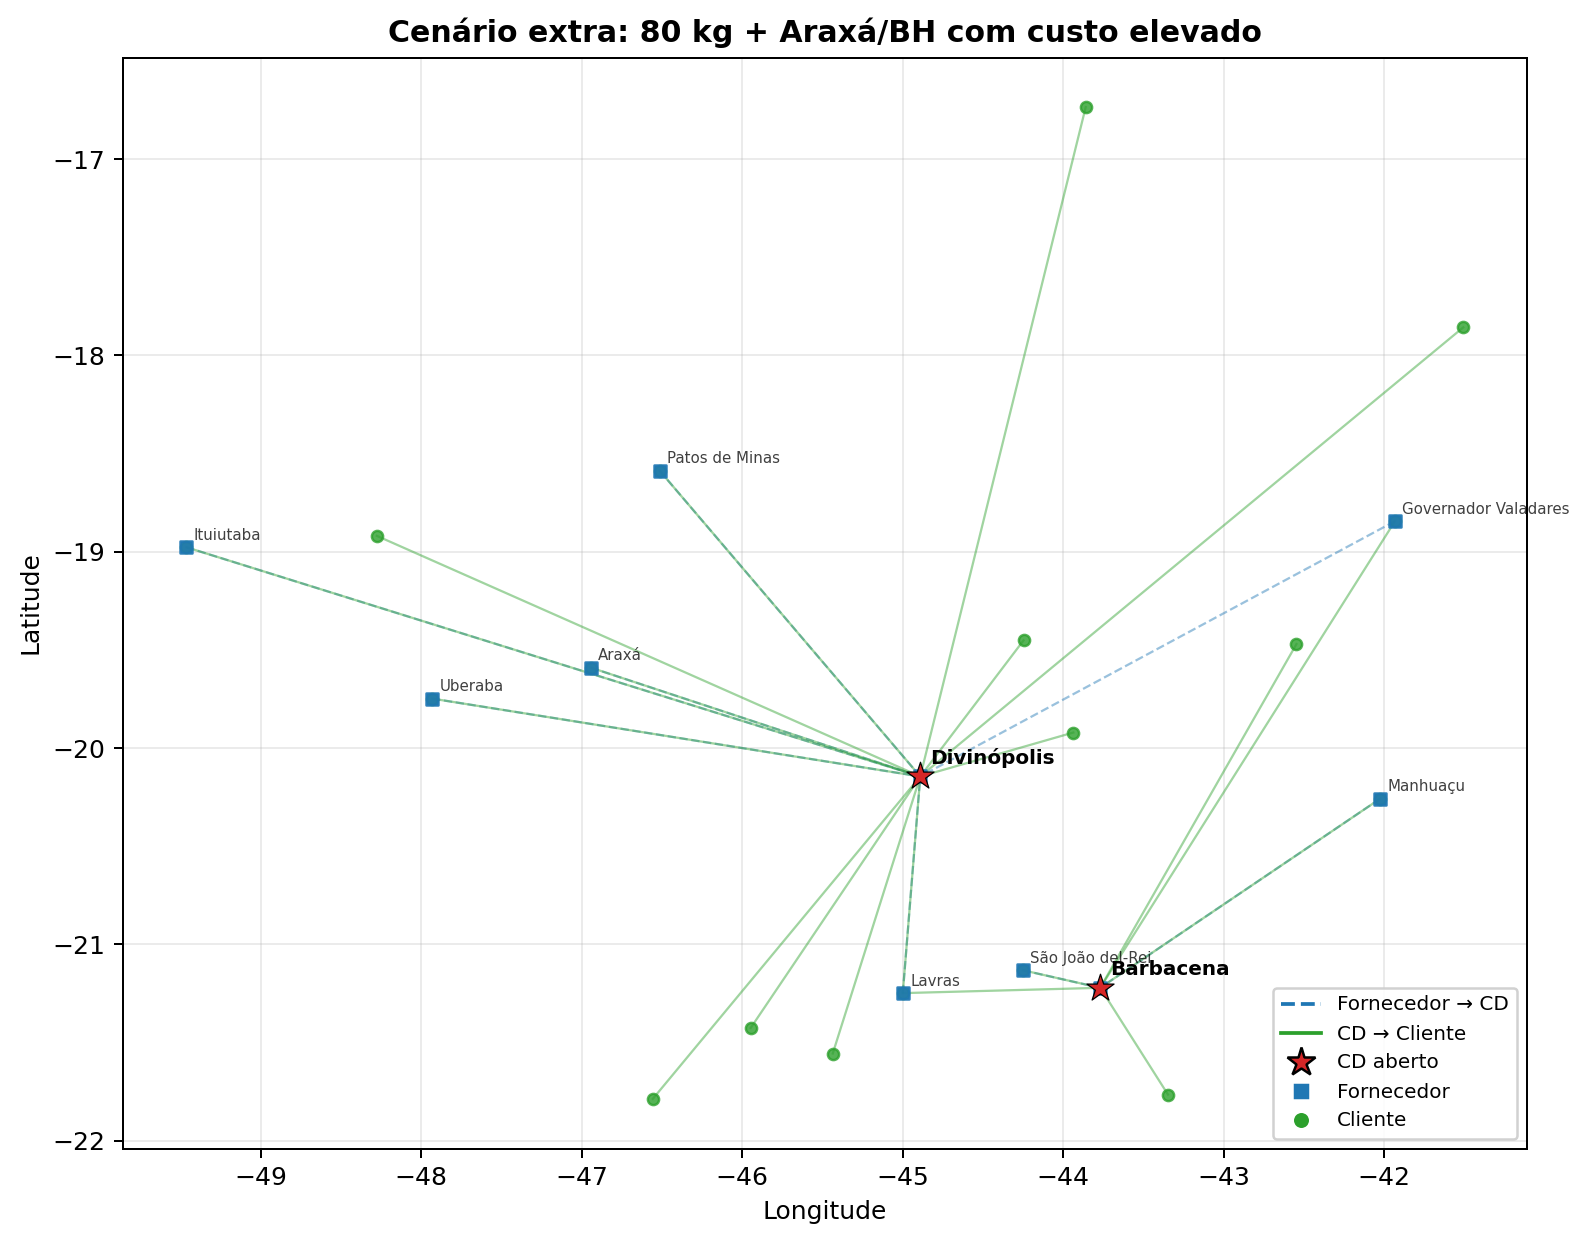
\includegraphics[width=0.95\textwidth]{imgs/mapa_cenario_extra_cap80_bh_araxa_caros.png}
\caption{Rotas geradas no cenário extra com caminhões de 80 kg e CDs centrais encarecidos}
\label{fig:mapa_cenario_extra}
\end{figure}

Nessa perspectiva, comparando os resultados, observa-se que o cenário extra produziu uma alteração mais significativa do que a simples redução da capacidade dos caminhões. Além de aumentar o número de viagens, a mudança nos custos de instalação alterou os CDs escolhidos e, consequentemente, a distribuição das rotas. O custo total ficou aproximadamente \textbf{38,24\%} maior que no Cenário 5 e \textbf{44,49\%} maior que no cenário base. Portanto, esse cenário evidencia que decisões logísticas são sensíveis não apenas à capacidade dos veículos, mas também à disponibilidade e ao custo de instalação dos centros de distribuição.

% =========================================
\section{Implementacao do modelo}
% =========================================

O modelo computacional utilizado no trabalho foi implementado em Python. A implementação foi estruturada para ler os dados de cada cenário a partir de planilhas no formato \texttt{.xlsx}, montar as variáveis de decisão, calcular os custos de transporte com base na distância geográfica entre as cidades, definir a função objetivo e aplicar as restrições do problema.

O código utiliza a fórmula de Haversine para estimar as distâncias entre fornecedores, candidatos a centros de distribuição e clientes. Em seguida, essas distâncias são combinadas com a capacidade dos caminhões para formar os custos de transporte. O problema é resolvido por meio da função \texttt{milp}, da biblioteca \texttt{scipy.optimize}, considerando variáveis contínuas para os fluxos e variáveis inteiras/binárias para as decisões de abertura de centros de distribuição e alocação de torrefadoras.

Como o mesmo modelo foi utilizado para todos os cenários, as diferenças entre as execuções ocorreram principalmente por meio da alteração dos parâmetros nas planilhas, como oferta, demanda, custos fixos, disponibilidade de torrefadoras e capacidade dos caminhões. Dessa forma, o código funcionou como uma base única para testar os diferentes cenários propostos



\nocite{*}

\bibliographystyle{apacite}
\bibliography{sample}

\end{document}